% ============================================================
%  The Particle Model — Lesson Booklet (one section per lesson: A Reading · B Theory · C Practice · D Above level)
%  Year 7 (Year 8 extension)  |  Victorian Curriculum F–10 Version 2.0
%  Compile with: xelatex three times, then python3 fill.py Particle_Model_Lesson_Booklet_Yr7
% ============================================================
\documentclass[11pt,a5paper,twoside]{article}
\newcommand{\wrcoverfile}{../../../covers/ecosystems.jpg}\newcommand{\unitname}{Biodiversity and Ecosystems}\newcommand{\unitcaps}{BIODIVERSITY AND ECOSYSTEMS}

% ── Fonts (compile with LuaLaTeX) ────────────────────────────────────────────
\usepackage{fontspec}
% Bundled fonts (in ./fonts/) so the document compiles anywhere with XeLaTeX/LuaLaTeX
\setmainfont{Lato}[                   % body — humanist sans (stands in for deck's Inter)
  Path=../fonts/, Extension=.ttf, Ligatures=TeX,
  UprightFont=Lato-Regular, ItalicFont=Lato-Italic,
  BoldFont=Lato-Bold, BoldItalicFont=Lato-BoldItalic ]
\newfontfamily\headingfont{Poppins}[  % display/headings — matches the slide decks
  Path=../fonts/, Extension=.ttf, Ligatures=TeX,
  UprightFont=Poppins-Regular, ItalicFont=Poppins-Italic,
  BoldFont=Poppins-Bold, BoldItalicFont=Poppins-BoldItalic ]
\setlength{\headheight}{22pt}

\usepackage[protrusion=true,expansion=false]{microtype}
\usepackage[a5paper, inner=17mm, outer=13mm, top=19mm, bottom=17mm, headheight=14pt, headsep=4mm, footskip=8mm]{geometry}
\usepackage{xcolor}
\usepackage{tikz}
\usetikzlibrary{arrows.meta, shapes.geometric, calc, positioning, decorations.pathreplacing}
\usepackage{tcolorbox}
\tcbuselibrary{skins, breakable, raster}
\usepackage{fancyhdr}
\usepackage{titlesec}
\usepackage{enumitem}
\usepackage{booktabs}
\usepackage{tabularx}
\usepackage{array}
\usepackage{colortbl}
\usepackage{multicol}
\usepackage{amsmath}
\usepackage{needspace}
% TikZ diagram macros are embedded below (just before \begin{document}) for easy editing.
\usepackage{longtable}
\usepackage{graphicx}
\usepackage{pifont}
\usepackage{lastpage}
\usepackage{calc}
\usepackage{mdframed}
\usepackage{setspace}
\usepackage{ragged2e}
% PDF bookmarks: one per lesson (made in \sectiondiv) plus the cover and
% contents, and links from the contents table to each lesson.
% implicit=false: hyperref adds no anchors of its own (an anchor on each
% list item nudged lists down 1.5 mm, which would undo the page fill).
% hidelinks keeps the links invisible, so the printed pages are unchanged.
\usepackage[implicit=false, hidelinks,
  pdftitle={Biodiversity and Ecosystems — Lesson Booklet},
  pdfsubject={Years 7–8 Science, Victorian Curriculum F–10 v2.0}]{hyperref}
\usepackage{bookmark} % writes the outline itself, which implicit=false switches off in hyperref
% hyperref 7.01 with implicit=false leaves \Hy@PageAnchorSlide undefined, which
% throws at \end{document} and stops fill.py (it builds with -halt-on-error).
\makeatletter\providecommand\Hy@PageAnchorSlide{}\makeatother

% ── Colour Palette ───────────────────────────────────────────────────────────
% Remapped to the slide-deck palette (names kept so body + diagrams cascade)
\definecolor{NavyBlue}   {HTML}{16305C}
\definecolor{MidBlue}    {HTML}{2E6FE0}
\definecolor{LightBlue}  {HTML}{E8F1FF}
\definecolor{TealGreen}  {HTML}{0F6E63}
\definecolor{LightGreen} {HTML}{E0F7F3}
\definecolor{GoldDark}   {HTML}{C77F12}
\definecolor{GoldLight}  {HTML}{FFF3DC}
\definecolor{PurpleDark} {HTML}{5B3FC0}
\definecolor{PurpleLight}{HTML}{EFE9FF}
\definecolor{OrangeDark} {HTML}{C9483D}
\definecolor{OrangeLight}{HTML}{FFE9E6}
\definecolor{MidGrey}    {HTML}{AEBED4}
\definecolor{LightGrey}  {HTML}{F2F5FA}
\definecolor{DarkGrey}   {HTML}{3A4759}
\definecolor{TableHead}  {HTML}{16305C}
\definecolor{RowAlt}     {HTML}{EEF4FF}
% Bright accent tints (deck) for bars, rules and chips
\definecolor{Blue}   {HTML}{2E6FE0}
\definecolor{Teal}   {HTML}{18A999}
\definecolor{Amber}  {HTML}{F5A623}
\definecolor{Coral}  {HTML}{FF6B5E}
\definecolor{Violet} {HTML}{7C5CE0}
\definecolor{Sky}    {HTML}{4DA3FF}
\definecolor{Ink}    {HTML}{16223A}
\definecolor{Line}   {HTML}{DDE5F0}
\definecolor{Paper}  {HTML}{FBFCFE}

% ── Page Style ───────────────────────────────────────────────────────────────
\pagestyle{fancy}
\fancyhf{}
\renewcommand{\headrulewidth}{0.4pt}
\renewcommand{\headrule}{\hbox to\headwidth{\color{NavyBlue}\leaders\hrule height \headrulewidth\hfill}}
\fancyhead[L]{\headingfont\small\color{NavyBlue}The Particle Model}
\fancyhead[R]{\headingfont\small\color{DarkGrey}Year 7 \textbar{} Victorian Curriculum F--10 v2.0}
\fancyfoot[C]{\headingfont\small\color{DarkGrey}\thepage\ \textbar{} \pageref{LastPage}}
\fancypagestyle{plain}{%
  \fancyhf{}
  \fancyfoot[C]{\headingfont\small\color{DarkGrey}\thepage\ \textbar{} \pageref{LastPage}}
  \renewcommand{\headrulewidth}{0pt}
}

% ── Section Formatting ───────────────────────────────────────────────────────
\titleformat{\section}
  {\headingfont\color{NavyBlue}\Large\bfseries}
  {}{0em}{}
  [{\color{Teal}\rule[0.6ex]{2.2em}{3pt}}{\color{Line}\rule[0.6ex]{\dimexpr\linewidth-2.2em\relax}{1pt}}]
\titlespacing{\section}{0pt}{18pt}{8pt}

\titleformat{\subsection}
  {\headingfont\color{MidBlue}\large\bfseries}
  {\thesubsection}{0.6em}{}
\titlespacing{\subsection}{0pt}{12pt}{4pt}

\titleformat{\subsubsection}
  {\headingfont\color{NavyBlue}\normalsize\bfseries}
  {}{0em}{}
\titlespacing{\subsubsection}{0pt}{8pt}{2pt}

% Deck-style eyebrow / kicker (optional use)
\newcommand{\kicker}[2][Teal]{%
  {\headingfont\bfseries\footnotesize\color{#1}%
   \textcolor{#1}{\rule[0.18ex]{1.6em}{2.2pt}}\hspace{0.5em}\MakeUppercase{#2}\par}%
  \vspace{2pt}}

% ── Custom tcolorbox Environments ────────────────────────────────────────────

% Section divider banner
\newtcolorbox{sectionbanner}[2]{
  enhanced, breakable=false,
  colback=NavyBlue, colframe=NavyBlue,
  fontupper=\color{white}\bfseries\large,
  left=4mm, right=4mm, top=3mm, bottom=3mm,
  title={\color{white}\Huge\bfseries #1},
  attach boxed title to top left={yshift=-2mm, xshift=4mm},
  boxed title style={colback=NavyBlue, colframe=NavyBlue},
  after upper={\par\smallskip\normalfont\normalsize\color{white!80!NavyBlue}\textit{#2}}
}

% Key info box (blue)
\newtcolorbox{infobox}[1]{
  breakable, arc=2.5mm, boxrule=0.5pt,
  colback=LightBlue, colframe=Blue!40,
  fonttitle=\headingfont\bfseries, coltitle=MidBlue,
  title={#1},
  left=4mm, right=3.5mm, top=2.5mm, bottom=2.5mm
}

% Scaffold box (yellow)
\newtcolorbox{scaffold}[1]{
  breakable, arc=2.5mm, boxrule=0.5pt,
  colback=GoldLight, colframe=Amber!40,
  fonttitle=\headingfont\bfseries, coltitle=GoldDark,
  title={#1},
  left=4mm, right=3.5mm, top=2.5mm, bottom=2.5mm
}

% Worked example box
\newtcolorbox{workedexbox}[1]{
  breakable, arc=2.5mm, boxrule=0.5pt,
  colback=white, colframe=Amber!50,
  fonttitle=\headingfont\bfseries, coltitle=GoldDark,
  title={#1},
  left=4mm, right=3.5mm, top=2.5mm, bottom=2.5mm
}
% Worked examples: \begin{workedex}{title} -> "Worked Example N.M --- title",
% auto-numbered per section and labelled we:N.M. Never type the number.
\newcounter{wenum}[section]
\renewcommand{\thewenum}{\thesection.\arabic{wenum}}
\newenvironment{workedex}[1]
  {\refstepcounter{wenum}\label{we:\thewenum}\begin{workedexbox}{Worked Example \thewenum\ --- #1}}
  {\end{workedexbox}}

% We do: straight after each worked example, a near-identical question the
% class works through together, with its own writing space. Numbered to
% match the worked example above it and labelled wd:N.M.
%   \begin{wedo}{title} question ... \answerbox{h} \end{wedo}
\newtcolorbox{wedobox}[1]{
  enhanced, breakable=false, arc=2.5mm, boxrule=0.5pt,
  colback=white, colframe=TealGreen!55,
  fonttitle=\headingfont\bfseries, coltitle=TealGreen!75!black,
  title={#1},
  left=4mm, right=3.5mm, top=2.5mm, bottom=2.5mm
}
\newenvironment{wedo}[1]
  {\par\needspace{9\baselineskip}\begin{wedobox}{We do \thewenum\ --- #1}\label{wd:\thewenum}\ignorespaces}
  {\end{wedobox}}

% Year 7 box (blue)
\newtcolorbox{yr7box}{
  breakable, arc=2.5mm, boxrule=0.5pt,
  colback=LightBlue, colframe=Blue!40,
  left=4mm, right=3.5mm, top=2.5mm, bottom=2.5mm
}

% Year 8 extension box (violet)
\newtcolorbox{yr8box}{
  breakable, arc=2.5mm, boxrule=0.5pt,
  colback=PurpleLight, colframe=Violet!40,
  left=4mm, right=3.5mm, top=2.5mm, bottom=2.5mm
}

% Answer lines box
\newcommand{\answerbox}[1]{%
  \begin{tcolorbox}[
    enhanced, breakable, arc=2mm,
    colback=Paper, colframe=Line,
    left=2mm, right=2mm, top=1mm, bottom=1mm,
    boxrule=1pt,
    height=#1
  ]
  \end{tcolorbox}%
}

% Experiment header
\newtcolorbox{expheader}[3]{
  breakable=false, arc=2.5mm,
  colback=RowAlt, colframe=Amber!50, boxrule=0.5pt,
  fonttitle=\headingfont\bfseries\large, coltitle=NavyBlue,
  title={Experiment #1: #2},
  left=4mm, right=3.5mm, top=2.5mm, bottom=2.5mm,
  after upper={\par\smallskip
    {\headingfont\bfseries\color{GoldDark}Aim:}\ \textit{#3}},
}

% Reading comprehension passage box (green)
\newtcolorbox{readingbox}[1]{
  breakable, arc=2.5mm, boxrule=0.5pt,
  colback=white, colframe=Teal!50,
  fonttitle=\headingfont\bfseries, coltitle=TealGreen,
  title={#1},
  left=4mm, right=3.5mm, top=2.5mm, bottom=2.5mm,
  fontupper=\normalsize
}

% Skill-builder box (for beginner scaffolding)
\newtcolorbox{skillbox}[1]{
  breakable, arc=2.5mm, boxrule=0.5pt,
  colback=RowAlt, colframe=Blue!40,
  fonttitle=\headingfont\bfseries, coltitle=MidBlue,
  title={#1},
  left=4mm, right=3.5mm, top=2.5mm, bottom=2.5mm
}

% ── Custom Commands ───────────────────────────────────────────────────────────

% Question: \question{marks}{text}  (marks can be empty)
% Numbered automatically as Q<section>.<n>, reset every section.
% Do NOT write numbers by hand.
\newcounter{qnum}[section]
\renewcommand{\theqnum}{\thesection.\arabic{qnum}}
\newcommand{\question}[2]{%
  \refstepcounter{qnum}%
  \needspace{3\baselineskip}%
  \medskip
  \noindent\label{q:\theqnum}\textbf{Q\theqnum}\ifx&#1&\else\ \textcolor{DarkGrey}{(#1 mark\ifnum#1=1\else s\fi)}\fi\quad #2%
  \medskip
}

% Inline marks note
\newcommand{\markscount}[1]{\hfill\textcolor{DarkGrey}{\textit{(#1 mark\ifnum#1=1\else s\fi)}}}

% ── Practice set counter and question macros ─────────────────────────────────
\newcounter{pqnum}
\newcommand{\practiceset}[1]{%
  \needspace{6\baselineskip}
  \setcounter{pqnum}{0}%
  \vspace{6pt}
  {\headingfont\bfseries\large\color{GoldDark} Practice Set --- #1}\\[-2pt]
  {\color{Amber}\rule{\linewidth}{1pt}}\\[2pt]
}
% \pq{question text}{working box height}
\newcommand{\pq}[2]{%
  \stepcounter{pqnum}%
  \needspace{4\baselineskip}
  \vspace{5pt}
  \noindent\textbf{\thepqnum.}\quad #1\par
  \vspace{2pt}
  \answerbox{#2}
}
% Two short questions side by side, each with its own box
\newcommand{\pqpair}[4]{%
  \needspace{4\baselineskip}
  \vspace{5pt}
  \noindent
  \begin{minipage}[t]{0.48\linewidth}
    \stepcounter{pqnum}\textbf{\thepqnum.}\quad #1\par\vspace{2pt}
    \begin{tcolorbox}[enhanced,arc=2mm,colback=Paper,colframe=Line,left=2mm,right=2mm,
      top=1mm,bottom=1mm,boxrule=1pt,height=#2]\end{tcolorbox}
  \end{minipage}\hfill
  \begin{minipage}[t]{0.48\linewidth}
    \stepcounter{pqnum}\textbf{\thepqnum.}\quad #3\par\vspace{2pt}
    \begin{tcolorbox}[enhanced,arc=2mm,colback=Paper,colframe=Line,left=2mm,right=2mm,
      top=1mm,bottom=1mm,boxrule=1pt,height=#4]\end{tcolorbox}
  \end{minipage}
}

% ── Comprehension question macro (compact, lined) ────────────────────────────
\newcounter{rcnum}
\newcommand{\rcreset}{\setcounter{rcnum}{0}}
\newcommand{\rcq}[2]{%
  \stepcounter{rcnum}%
  \needspace{3\baselineskip}
  \vspace{4pt}
  \noindent\textbf{C\thercnum.}\quad #1\par
  \vspace{2pt}
  \linedbox{#2}
}

% Section divider (big numbered banner): \sectiondiv{title}{summary}
%
% This IS the section: it steps the real section counter, so subsections,
% tasks, questions and figures inside it are numbered N.M automatically.
% Put \label{sec:N} straight after it. Never hand-type a section number.
\newcommand{\sectiondiv}[2]{%
  \needspace{5\baselineskip}%
  \refstepcounter{section}%
  % PDF bookmark for the lesson; its anchor, lesson.N.1, is what the contents table links to
  \pdfbookmark[1]{Lesson \thesection{} — #1}{lesson.\thesection}%
  \begin{tcolorbox}[
    enhanced, breakable=false, arc=3.5mm,
    colback=NavyBlue, colframe=NavyBlue, boxrule=0pt,
    sidebyside, sidebyside align=center,
    lefthand width=2.4cm,
    left=2mm, right=4mm, top=4mm, bottom=4mm
  ]
    \begin{center}
      {\headingfont\bfseries\color{white!35!NavyBlue}\fontsize{50}{50}\selectfont \thesection}
    \end{center}
    \tcblower
    {\headingfont\bfseries\color{white}\LARGE #1}\\[3pt]
    {\itshape\color{white!75!NavyBlue}\small #2}
  \end{tcolorbox}%
}

% Tasks: \task, \task[a] (part a of a NEW task), \taskpart{b} (next part
% of the same task), \exttask (Year 8 "Extension" — same counter).
% Numbered Task <section>.<n>, reset every section. Do NOT type numbers.
% Every task, question and figure also gets an automatic label
% (task:1.7b, q:2.4, fig:1.2, fig:E2.1) so page refs come from the .aux.
\newcounter{tasknum}[section]
\renewcommand{\thetasknum}{\thesection.\arabic{tasknum}}
\NewDocumentCommand{\task}{o}{\refstepcounter{tasknum}\label{task:\thetasknum\IfValueT{#1}{#1}}\textbf{Task \thetasknum\IfValueT{#1}{#1}}}
\newcommand{\taskpart}[1]{\label{task:\thetasknum#1}\textbf{Task \thetasknum#1}}
\newcommand{\exttask}{\refstepcounter{tasknum}\label{task:\thetasknum}\textbf{Extension \thetasknum}}

% Figure captions: \figcap[fig:label]{caption} -> "Figure N.M --- caption"
% \expfigcap{caption} -> "Figure EN.M" (experiment pages). Both auto-numbered.
\newcounter{fignum}[section]
\renewcommand{\thefignum}{\thesection.\arabic{fignum}}
\newcounter{expfignum}[section]
\renewcommand{\theexpfignum}{E\thesection.\arabic{expfignum}}
\newcommand{\figcap}[2][]{%
  \begin{center}
    \refstepcounter{fignum}\label{fig:\thefignum}\if\relax\detokenize{#1}\relax\else\label{#1}\fi
    \small\itshape\color{DarkGrey} Figure \thefignum\ --- #2
  \end{center}%
}
\newcommand{\expfigcap}[1]{%
  \begin{center}
    \refstepcounter{expfignum}\label{fig:\theexpfignum}%
    \small\itshape\color{DarkGrey} Figure \theexpfignum\ --- #1
  \end{center}%
}

% Diagram include
\newcommand{\diagramfig}[3]{%  {filename}{width fraction}{caption}
  \begin{center}
    \includegraphics[width=#2\linewidth]{#1}\\[4pt]
    \small\itshape\color{DarkGrey} #3
  \end{center}%
}

% Table column types
\newcolumntype{L}[1]{>{\RaggedRight\arraybackslash}p{#1}}
\newcolumntype{C}[1]{>{\Centering\arraybackslash}p{#1}}

% Table header colour
\newcommand{\thead}[1]{\cellcolor{TableHead}\color{white}\bfseries #1}
\newcommand{\talt}{\rowcolor{RowAlt}}
\newcommand{\tmid}{\rowcolor{MidGrey}}

% Inline year tags
\newcommand{\tagyr}[1]{%
  \tikz[baseline=-0.5ex]\node[
    rounded corners=2pt,
    fill=#1!20, draw=#1, text=#1,
    inner xsep=4pt, inner ysep=1pt,
    font=\scriptsize\bfseries
  ]{Yr #1 only};}

% Draw answer lines
\newcommand{\anslines}[1]{%
  \vspace{2pt}%
  \foreach \n in {1,...,#1}{%
    \par\noindent\rule{\linewidth}{0.3pt}\vspace{3pt}%
  }%
}

% ── Document ─────────────────────────────────────────────────────────────────
% ── Optional-lesson note, shown under the lesson banner ──────────────────────
\newcommand{\optionalnote}[1]{%
  % the title is a bold lead-in on the first line rather than a title bar,
  % which keeps Lesson 11's reading on the lesson's first page
  \begin{tcolorbox}[enhanced, breakable=false, arc=2.5mm, boxrule=0.5pt,
    colback=PurpleLight, colframe=Violet!50,
    left=4mm, right=3.5mm, top=2mm, bottom=2mm]
  {\headingfont\bfseries\color{PurpleDark}Optional lesson \textbullet{} Year 8 extension.}\enspace #1
  \end{tcolorbox}\vspace{2pt}}


% ══════════════════════════════════════════════════════════════════════════════
%  LESSON STRUCTURE (lesson booklet, Oct 2026)
%  Every lesson runs in the same four parts, in this order:
%    \lessonpart{A}{Reading and comprehension}{Teal}   \label{read:N}
%    \lessonpart{B}{Theory and examples}{Blue}         \label{theory:N}
%    \lessonpart{C}{Practice}{Amber}                    \label{prac:N}
%    \lessonpart{D}{Above level}{Violet}                \label{ext:N}
%  Above-level / higher-order questions live ONLY in Part D, at the end.
% ══════════════════════════════════════════════════════════════════════════════
\newcommand{\lessonpart}[3]{%
  \par\if#1A\needspace{10\baselineskip}\vspace{10pt}\else
    \if#1C\notesfill\fi\clearpage\fi
  \begin{tcolorbox}[enhanced, breakable=false, arc=2mm, boxrule=0pt,
    colback=#3!14, borderline west={4pt}{0pt}{#3},
    left=4mm, right=3mm, top=1.6mm, bottom=1.6mm]
  {\headingfont\bfseries\color{#3!60!black}\large Part #1 \textbullet{} #2}
  \end{tcolorbox}\vspace{2pt}}

% Key vocabulary at the start of each lesson: students copy each definition
% from the vocabulary slide in the lesson's starter. First row = red scaffold.
\newcommand{\vocabhead}{%
  \par\vspace{6pt}%
  \begin{tcolorbox}[enhanced, breakable=false, arc=2mm, boxrule=0pt,
    colback=NavyBlue!10, borderline west={4pt}{0pt}{NavyBlue},
    left=4mm, right=3mm, top=1.6mm, bottom=1.6mm]
  {\headingfont\bfseries\color{NavyBlue}\large Key vocabulary}
  \end{tcolorbox}\vspace{2pt}%
  \noindent Copy the definition of each word from the slide. The first one has been done for you.\par}

% Curriculum codes under a lesson banner
\newcommand{\lessoncodes}[1]{%
  {\small\headingfont\color{DarkGrey}Victorian Curriculum 2.0:\ \textbf{#1}}\par\vspace{4pt}}

% Two short tasks side by side, each with its own working box
% \taskpair{text}{box height}{text}{box height}
% The two boxes line up: the shorter question is padded by the difference in
% text height (measured in a scratch box, task counter restored, no label).
\newsavebox\tpbox
\newlength\tpA \newlength\tpB
\newcount\tpsaved
\newcommand\tpmeasure[2]{%
  \tpsaved=\value{tasknum}%
  \sbox\tpbox{\vbox{\hsize=0.485\linewidth \linewidth=\hsize \parskip=0pt
    \renewcommand\label[1]{}\task #1\par}}%
  \setlength{#2}{\dimexpr\ht\tpbox+\dp\tpbox\relax}%
  \setcounter{tasknum}{\tpsaved}}
\newcommand{\taskpair}[4]{%
  \par\needspace{9\baselineskip}\vspace{4pt}%
  \tpmeasure{#1}{\tpA}\tpmeasure{#3}{\tpB}%
  \noindent
  \edef\abgrp{\number\numexpr\value{abox}+1\relax}%
  \begin{minipage}[t]{0.485\linewidth}
    \task #1\par\ifdim\tpB>\tpA\vspace{\dimexpr\tpB-\tpA\relax}\fi\vspace{2pt}\answerbox{#2}
  \end{minipage}\hfill
  \begin{minipage}[t]{0.485\linewidth}
    \task #3\par\ifdim\tpA>\tpB\vspace{\dimexpr\tpA-\tpB\relax}\fi\vspace{2pt}\answerbox{#4}
  \end{minipage}\par\gdef\abgrp{0}\vspace{4pt}}
% Two parts of one question side by side, with their answer boxes level:
% \ptpair{a}{part (a) text}{box height}{b}{part (b) text}{box height}.
% The shorter part's text gets space below it to match the longer one.
\newcommand\ptmeasure[3]{%
  \sbox\tpbox{\vbox{\hsize=0.485\linewidth \linewidth=\hsize \parskip=0pt \pt{#1}#2\par}}%
  \setlength{#3}{\dimexpr\ht\tpbox+\dp\tpbox\relax}}
\newcommand{\ptpair}[6]{%
  \ptmeasure{#1}{#2}{\tpA}\ptmeasure{#4}{#5}{\tpB}%
  \par\noindent
  \edef\abgrp{\number\numexpr\value{abox}+1\relax}%
  \begin{minipage}[t]{0.485\linewidth}
    \pt{#1}#2\par\ifdim\tpB>\tpA\vspace{\dimexpr\tpB-\tpA\relax}\fi\answerbox{#3}
  \end{minipage}\hfill
  \begin{minipage}[t]{0.485\linewidth}
    \pt{#4}#5\par\ifdim\tpA>\tpB\vspace{\dimexpr\tpA-\tpB\relax}\fi\answerbox{#6}
  \end{minipage}\par\gdef\abgrp{0}}

% Answer boxes never split across a page (a half box on its own page is useless)
% ── Page filling ────────────────────────────────────────────────────────────
% Every writing box gets an id. Its page is logged to \jobname.abp; fill.py
% measures the empty space left at the foot of each page and shares it out
% among that page's boxes via \jobname.abx (\abset{id}{extra}). Side-by-side
% boxes share a group so they grow together.
\newcounter{abox}
\newwrite\abpos \immediate\openout\abpos=\jobname.abp
\newcommand{\abset}[2]{\expandafter\gdef\csname abx@#1\endcsname{#2}}
\InputIfFileExists{\jobname.abx}{}{}
\def\abgrp{0}
\newcommand{\abnext}{\stepcounter{abox}%
  \edef\abcur{\ifcsname abx@\theabox\endcsname\csname abx@\theabox\endcsname\else 0pt\fi}}
\newcommand{\ablog}{\edef\abtmp{\noexpand\write\abpos{\theabox\space\abgrp\space\noexpand\thepage}}\abtmp}
\newcommand{\abh}[1]{\dimexpr#1+\abcur\relax}
\renewcommand{\answerbox}[1]{%
  \abnext
  \begin{tcolorbox}[enhanced, breakable=false, arc=2mm, colback=Paper, colframe=Line,
    left=2mm, right=2mm, top=1mm, bottom=1mm, boxrule=1pt, height=\abh{#1}]
  \end{tcolorbox}\ablog%
}
% \linedbox{height}: an answer box ruled in dotted thirds. Lines are \thirdrow/3 apart and run dotted, dotted,
% solid (the baseline), repeating, and end on one dotted line. The number of
% rows is worked out from the box's final height, so the ruling still fills the
% box after fill.py has grown it; the rows are centred in the box.
\newlength\thirdrow \setlength\thirdrow{9mm}
\tikzset{thirdsolid/.style={draw=DarkGrey!70, line width=0.5pt},
         thirddot/.style={draw=DarkGrey!70, line width=0.6pt, dash pattern=on 0.9pt off 1.6pt}}
\newlength\lbH \newlength\lbO \newcount\lbN
\newcommand{\linedbox}[1]{%
  \abnext
  % interior height = box height less the 1pt frame top and bottom
  \setlength\lbH{\dimexpr\abh{#1}-2pt\relax}%
  % whole rows that fit with at least 3 mm spare top and bottom (at least one)
  \lbN=\numexpr(\dimexpr\lbH-6mm-\thirdrow/2\relax)/\thirdrow\relax
  \ifnum\lbN<1 \lbN=1 \fi
  \setlength\lbO{\dimexpr(\lbH-\lbN\thirdrow)/2\relax}%
  \begin{tcolorbox}[enhanced, breakable=false, arc=2mm, colback=Paper, colframe=Line,
    left=2mm, right=2mm, top=1mm, bottom=1mm, boxrule=1pt, height=\abh{#1},
    underlay={\begin{tcbclipinterior}
      \foreach \i in {1,...,\the\lbN}{
        \draw[thirddot] ([xshift=3mm,yshift=-\lbO-(\i-1)*\thirdrow]interior.north west) -- ([xshift=-3mm,yshift=-\lbO-(\i-1)*\thirdrow]interior.north east);
        \draw[thirddot] ([xshift=3mm,yshift=-\lbO-(\i-1)*\thirdrow-\thirdrow/3]interior.north west) -- ([xshift=-3mm,yshift=-\lbO-(\i-1)*\thirdrow-\thirdrow/3]interior.north east);
        \draw[thirdsolid] ([xshift=3mm,yshift=-\lbO-(\i-1)*\thirdrow-2*\thirdrow/3]interior.north west) -- ([xshift=-3mm,yshift=-\lbO-(\i-1)*\thirdrow-2*\thirdrow/3]interior.north east);}
      \draw[thirddot] ([xshift=3mm,yshift=-\lbO-\lbN\thirdrow]interior.north west) -- ([xshift=-3mm,yshift=-\lbO-\lbN\thirdrow]interior.north east);
    \end{tcbclipinterior}}]
  \end{tcolorbox}\ablog%
}
% Every written-response box is ruled the same way (Part A comprehension, We do,
% Part C tasks and Part D extensions, including side-by-side pairs). Space for
% mathematical working uses \workbox{height} instead and stays plain, as do
% \drawbox and the write-in tables.
\let\workbox\answerbox   % plain box: mathematical working (calculations) stays unruled
\let\answerbox\linedbox
% \drawbox{height}{contents}: white box for a diagram or drawing
\newcommand{\drawbox}[2]{%
  \abnext
  \begin{tcolorbox}[colback=white, colframe=MidGrey, boxrule=0.5pt, height=\abh{#1}]#2\end{tcolorbox}\ablog}
% Notes box at the end of Part B: fills whatever is left of the page (if worth it)
\newcommand{\notesfill}{\par
  \ifdim\dimexpr\pagegoal-\pagetotal\relax>3.2cm
    \vspace*{\fill}%
    \begin{tcolorbox}[enhanced, breakable=false, arc=2mm, colback=Paper, colframe=Line,
      left=2mm, right=2mm, top=1mm, bottom=1mm, boxrule=1pt,
      height=\dimexpr\pagegoal-\pagetotal-1.0cm\relax]
      {\small\headingfont\color{DarkGrey}Notes}
    \end{tcolorbox}%
  \fi}



% Centred table: wrap every content table in \begin{ctab} ... \end{ctab}
% (figures already centre themselves inside their \diag... macros)
% ctab also registers write-in tables (S column) for page filling: the extra
% height is per row, logged with the row count.
\newenvironment{ctab}{\par\smallskip\begingroup\centering
  \abnext\let\tbcur\abcur\global\wtrows0 }{\par
  \ifnum\wtrows>0 \edef\abtmp{\noexpand\write\abpos{\theabox\space\abgrp\space\noexpand\thepage\space\the\wtrows}}\abtmp\fi
  \endgroup\smallskip}

% ── Booklet formatting rules (Oct 2026) ─────────────────────────────────────
% 1. No marks are shown anywhere in the booklet.
\renewcommand{\markscount}[1]{}
% 2. A task's heading sits on its own line; its text starts on the next
%    line, left aligned. Parts (a), (b)… each start a new line: use \pt{a}.
\RenewDocumentCommand{\task}{o}{\par\noindent\refstepcounter{tasknum}\label{task:\thetasknum\IfValueT{#1}{#1}}\textbf{Task \thetasknum\IfValueT{#1}{#1}}\par\nobreak\noindent\ignorespaces}
\renewcommand{\taskpart}[1]{\par\noindent\label{task:\thetasknum#1}\textbf{Task \thetasknum#1}\par\nobreak\noindent\ignorespaces}
\renewcommand{\exttask}{\par\noindent\refstepcounter{tasknum}\label{task:\thetasknum}\textbf{Extension \thetasknum}\par\nobreak\noindent\ignorespaces}
\newcommand{\pt}[1]{\par\noindent\textbf{(#1)}\ \ignorespaces}
% Workstation pages (Experiment 1): numbered method steps with a hanging
% indent, and a one-line safety reminder under the materials list.
\newcommand{\wsstep}[1]{\par\noindent\hangindent=1.6em\hangafter=1\makebox[1.6em][l]{\textbf{#1}}\ignorespaces}
\newcommand{\wssafety}[1]{\par\smallskip{\small\textcolor{ScaffoldRed}{\headingfont\bfseries Safety:}\ #1}\par}
% 3. Tables have vertical rules between columns and down both sides
%    (write | between and around the columns, e.g. {|L{3cm}|C{2cm}|}).
%    Keep the normal padding at the outer edges (no @{} there): colortbl paints
%    header colour one \tabcolsep past each edge, so trimming the padding makes
%    the header overhang the grid.
\arrayrulecolor{MidGrey}
\setlength{\arrayrulewidth}{0.6pt}
% 4. Write-in tables: W/Z are left/centred columns that centre text
%    vertically; put the S column first (see below).
\newcolumntype{W}[1]{>{\RaggedRight\arraybackslash}m{#1}}
\newcolumntype{Z}[1]{>{\Centering\arraybackslash}m{#1}}
\def\tbcur{0pt}
\newcount\wtrows
\newcommand{\wh}{\global\advance\wtrows1 \rule[\dimexpr-0.75cm-\tbcur/2\relax]{0pt}{\dimexpr1.5cm+\tbcur\relax}}
% S = zero-width first column that makes every row of a write-in table
% at least 1.5 cm tall with its text vertically centred. Start each data
% row with "&"; start the header row with "\hd &" so it stays slim.
\newif\ifnowh
\newcolumntype{S}{@{}>{}c<{\ifnowh\else\wh\fi\global\nowhfalse}@{\hspace{\tabcolsep}}}
\newcommand{\hd}{\global\nowhtrue}
% 5. The first row of a multi-row write-in table is a worked scaffold in red.
\definecolor{ScaffoldRed}{HTML}{C0392B}
\newcommand{\scaf}[1]{\textcolor{ScaffoldRed}{\itshape #1}}
% 6. Tables are a light grid (rules between rows and columns) on white —
%    row shading is off, because colortbl paints shading over column rules.
\renewcommand{\talt}{}
\renewcommand{\tmid}{}
% ══════════════════════════════════════════════════════════════════════════════
%  DIAGRAM DEFINITIONS — The Particle Model
%  Self-contained TikZ macros, no external image files. Each \diag... macro is
%  called from the body by name.
% ══════════════════════════════════════════════════════════════════════════════
\usetikzlibrary{arrows.meta,calc,positioning,patterns,backgrounds}
\tikzset{
  thin arrow/.style={-{Stealth[length=6pt,width=4pt]}, line width=1.4pt},
}

% ── Lesson 1: the same three jars holding a solid, a liquid and a gas ───────────
% The solid keeps its own shape, the liquid takes the jar's shape with a flat top,
% the gas fills the whole jar. No particles yet: those arrive in Lesson 4.
\newcommand{\jar}[1]{% jar outline with its base at (#1,0)
  \draw[line width=1.2pt, Ink] (#1-1.25,2.9) -- (#1-1.25,0.15) arc (180:270:0.15)
    -- (#1+1.1,0) arc (270:360:0.15) -- (#1+1.25,2.9);}
\newcommand{\diagStates}{%
\begin{center}
\begin{tikzpicture}[font=\small, x=1cm, y=1cm]
  % solid: a block sitting in the corner
  \fill[GoldLight] (-0.95,0.02) rectangle (0.15,1.25);
  \draw[GoldDark, line width=1.1pt] (-0.95,0.02) rectangle (0.15,1.25);
  \jar{0}
  \node[font=\bfseries, text=NavyBlue] at (0,-0.45) {Solid};
  \node[align=center, font=\footnotesize, text=DarkGrey] at (0,-1.05) {keeps its own shape\\and volume};
  % liquid: takes the jar's shape, flat top
  \begin{scope}[xshift=4.2cm]
    \fill[Sky!35] (-1.25,0.15) arc (180:270:0.15) -- (1.1,0) arc (270:360:0.15) -- (1.25,1.1) -- (-1.25,1.1) -- cycle;
    \draw[MidBlue, line width=1.1pt] (-1.25,1.1) -- (1.25,1.1);
    \jar{0}
    \node[font=\bfseries, text=NavyBlue] at (0,-0.45) {Liquid};
    \node[align=center, font=\footnotesize, text=DarkGrey] at (0,-1.05) {takes the jar's shape,\\keeps its volume};
  \end{scope}
  % gas: fills the whole (sealed) jar
  \begin{scope}[xshift=8.4cm]
    \fill[Violet!16] (-1.25,0.15) arc (180:270:0.15) -- (1.1,0) arc (270:360:0.15) -- (1.25,2.9) -- (-1.25,2.9) -- cycle;
    \draw[line width=2.2pt, DarkGrey] (-1.4,2.9) -- (1.4,2.9);
    \jar{0}
    \node[font=\scriptsize, text=DarkGrey, anchor=south] at (0,2.95) {lid};
    \node[font=\bfseries, text=NavyBlue] at (0,-0.45) {Gas};
    \node[align=center, font=\footnotesize, text=DarkGrey] at (0,-1.05) {spreads out to fill\\the whole jar};
  \end{scope}
\end{tikzpicture}
\end{center}}

% ── Lesson 1, Worked Example 1.2 and We do 1.2: the same syringe, before and after
\newcommand{\diagSyringe}[3]{% {start mL}{end mL}{contents: gas|liquid}
\begin{center}\resizebox{\linewidth}{!}{%
\begin{tikzpicture}[font=\scriptsize, x=0.11cm, y=1cm]
  \foreach \row/\vol/\lab in {0/#1/before, -1.15/#2/after}{
    \begin{scope}[yshift=\row cm]
      \ifx#3g\fill[Violet!16] (0,0) rectangle (\vol,0.7);\else\fill[Sky!35] (0,0) rectangle (\vol,0.7);\fi
      \draw[line width=1pt, Ink] (0,0) rectangle (60,0.7);
      \draw[line width=1pt, Ink] (0,0.25) -- (-4,0.25) (0,0.45) -- (-4,0.45);
      \fill[Ink] (-5.5,0.15) rectangle (-4,0.55);
      \foreach \t in {0,10,...,60}{\draw[Ink] (\t,0.7) -- (\t,0.85); \node[anchor=south, font=\tiny] at (\t,0.82) {\t};}
      \fill[DarkGrey] (\vol,0.04) rectangle (\vol+1.6,0.66);
      \draw[line width=2pt, DarkGrey] (\vol+1.6,0.35) -- (\vol+26,0.35);
      \draw[line width=2pt, DarkGrey] (\vol+26,0.05) -- (\vol+26,0.65);
      \node[anchor=east, font=\scriptsize\bfseries, text=DarkGrey] at (-7,0.35) {\lab};
    \end{scope}}
  \node[font=\tiny, text=DarkGrey, anchor=west] at (61,0.35) {mL};
  \node[font=\tiny, text=DarkGrey, anchor=north] at (-4.75,-1.2) {sealed tip};
\end{tikzpicture}}
\end{center}}

% needspace.sty reserves room by planting a penalty -100 with 9 lines of
% temporary stretch. On a page that can't be filled tightly that fake break
% always wins, so a We do that fitted was pushed over and left half a page
% empty. This version breaks only when the room really isn't there, and
% ragged bottom lets every other page run on until something won't fit;
% fill.py then grows the writing boxes into what is left at the foot.
\renewcommand{\needspace}[1]{\par\ifdim\dimexpr\pagegoal-\pagetotal\relax<\dimexpr#1\relax\newpage\fi}
\raggedbottom
% Part D sits in a breakable yr8box, where \needspace can't see the page (the box
% is built off the page first). Wrap each extension in keepext so it is one
% unsplittable block: the yr8box then breaks between extensions, never inside one.
\newenvironment{keepext}{\par\begin{tcolorbox}[blankest, breakable=false]}{\end{tcolorbox}\par}
\usetikzlibrary{patterns}
\providecommand{\lessonart}{\thesection}

\providecommand{\unitname}{Biodiversity and Ecosystems}\providecommand{\unitcaps}{BIODIVERSITY AND ECOSYSTEMS}
% ══════════════════════════════════════════════════════════════════════════════
%  2027 WORKBOOK STYLE — A5 LESSON BOOKLET (added by make_a5.py)
%  Same look as the Space A5 trial and the A4 experiment booklets: colour
%  cover, black-and-white inside, Outfit headings, a lesson opener band with
%  the lesson's ink symbol, boxes told apart by frame and icon:
%    I do ● solid · We do ●● dashed · You do ●●● heavy · key idea / reading ◆
%    thin · Above level ▲ double · Country ◎ dotted
%  The body still names the master's colours; they are mapped to ink here.
% ══════════════════════════════════════════════════════════════════════════════
\usepackage{pdflscape}
\usetikzlibrary{patterns}

% A picture wider than the A5 text block is scaled down to fit it.
\newsavebox\fitb
\newenvironment{fitbox}{\begin{lrbox}{\fitb}}{\end{lrbox}%
  \ifdim\wd\fitb>\linewidth\resizebox{\linewidth}{!}{\usebox\fitb}\else\usebox\fitb\fi}

% ── Fonts: Outfit for headings ──────────────────────────────────────────────
\renewfontfamily\headingfont{Outfit}[
  Path=../fonts/, Extension=.ttf, Ligatures=TeX,
  UprightFont=Outfit-Regular, BoldFont=Outfit-SemiBold,
  ItalicFont=Outfit-Regular, ItalicFeatures={FakeSlant=0.18},
  BoldItalicFont=Outfit-SemiBold, BoldItalicFeatures={FakeSlant=0.18} ]

% ── Black and white inside ──────────────────────────────────────────────────
\definecolor{Ink}{HTML}{111111}
\colorlet{NavyBlue}{Ink}\colorlet{MidBlue}{Ink}\colorlet{TealGreen}{Ink}
\colorlet{GoldDark}{Ink}\colorlet{PurpleDark}{Ink}\colorlet{OrangeDark}{Ink}
\colorlet{TableHead}{Ink}
\colorlet{Blue}{Ink}\colorlet{Teal}{Ink}\colorlet{Amber}{Ink}\colorlet{Coral}{Ink}
\colorlet{Violet}{Ink}\colorlet{Sky}{Ink}
\colorlet{LightBlue}{white}\colorlet{LightGreen}{white}\colorlet{GoldLight}{white}
\colorlet{PurpleLight}{white}\colorlet{OrangeLight}{white}\colorlet{RowAlt}{white}
\colorlet{LightGrey}{white}\colorlet{Paper}{white}
\colorlet{DarkGrey}{black!72}\colorlet{MidGrey}{black!45}\colorlet{Line}{black!45}
\arrayrulecolor{black!60}
% Particle kinds stay distinguishable without colour: white, light grey,
% dotted and dark.
\tikzset{
  pA/.style={circle, fill=white, draw=Ink, line width=0.6pt, minimum size=3.2mm, inner sep=0pt},
  pB/.style={circle, fill=black!35, draw=Ink, line width=0.6pt, minimum size=3.2mm, inner sep=0pt},
  pC/.style={circle, preaction={fill=white}, pattern=dots, draw=Ink, line width=0.6pt, minimum size=3.2mm, inner sep=0pt},
  pD/.style={circle, fill=black!75, draw=Ink, line width=0.6pt, minimum size=3.2mm, inner sep=0pt}}

% ── Page style: mirrored, running head on the outside ───────────────────────
\fancypagestyle{fancy}{\fancyhf{}%
  \renewcommand{\headrulewidth}{0.4pt}%
  \renewcommand{\headrule}{\hbox to\headwidth{\color{Ink}\leaders\hrule height \headrulewidth\hfill}}%
  \fancyhead[LE]{\headingfont\footnotesize \unitname}%
  \fancyhead[RO]{\headingfont\footnotesize\leftmark}%
  \fancyfoot[LE,RO]{\headingfont\footnotesize\thepage}}
\fancypagestyle{plain}{\fancyhf{}\renewcommand{\headrulewidth}{0pt}%
  \fancyfoot[LE,RO]{\headingfont\footnotesize\thepage}}
\fancypagestyle{opener}{\fancyhf{}\renewcommand{\headrulewidth}{0pt}%
  \fancyfoot[LE,RO]{\headingfont\footnotesize\thepage}}
\pagestyle{fancy}\markboth{}{}
\raggedbottom
\setlength{\emergencystretch}{2em}

\titleformat{\subsection}{\headingfont\large\bfseries}{\thesubsection}{0.6em}{}
\titleformat{\subsubsection}{\headingfont\normalsize\bfseries}{}{0em}{}

% ── Lesson opener band (replaces the navy section banner) ────────────────────
\renewcommand{\sectiondiv}[2]{%
  \clearpage\thispagestyle{opener}%
  \refstepcounter{section}\markboth{\thesection\ \textbullet\ #1}{\thesection\ \textbullet\ #1}%
  \pdfbookmark[1]{Lesson \thesection{} — #1}{lesson.\thesection}\hypertarget{lesson.\thesection.1}{}%
  \noindent\begin{minipage}[b]{\dimexpr\linewidth-36mm\relax}
    {\headingfont\bfseries\scriptsize\addfontfeatures{LetterSpace=14}\unitcaps\ \textbullet\ LESSON}\par\vspace{1mm}
    {\headingfont\bfseries\fontsize{40}{40}\selectfont\thesection}\par\vspace{1.5mm}
    {\headingfont\bfseries\fontsize{15}{18}\selectfont\RaggedRight #1\par}\vspace{1mm}
    {\footnotesize\itshape\RaggedRight #2\par}
  \end{minipage}\hfill
  \begin{minipage}[b]{34mm}\includegraphics[width=34mm]{../art/l\lessonart-ink.pdf}\end{minipage}\par
  \vspace{2.5mm}\noindent\rule{\linewidth}{1.6pt}\par\vspace{1mm}}
\renewcommand{\lessoncodes}[1]{{\small\itshape VC 2.0: #1}\par\vspace{2pt}}

% Lesson parts: a heading and a rule; B, C and D start a new page.
\renewcommand{\lessonpart}[3]{%
  \par\if#1A\needspace{10\baselineskip}\vspace{8pt}\else
    \if#1C\notesfill\fi\clearpage\fi
  {\headingfont\bfseries\Large Part #1 \textbullet\ #2}\par\vspace{0.5mm}\noindent\rule{\linewidth}{0.6pt}\par\vspace{1mm}}
\renewcommand{\vocabhead}{%
  \par\vspace{4pt}{\headingfont\bfseries\Large Key vocabulary}\par\vspace{1pt}%
  \noindent{\small Copy the meaning of each word from the slide. The first one has been done for you.}\par}
\renewcommand{\thead}[1]{\headingfont\bfseries #1}

% ── Box system ──────────────────────────────────────────────────────────────
\newcommand{\icodots}[1]{\tikz[baseline=-0.6ex]{\foreach \k in {1,...,#1}{\fill[white] (\k*1.9mm,0) circle (0.7mm);}}}
\newcommand{\icokey}{\tikz[baseline=-0.6ex]{\fill[white] (0,0.9mm)--(0.9mm,0)--(0,-0.9mm)--(-0.9mm,0)--cycle;}}
\newcommand{\icoup}{\tikz[baseline=-0.6ex]{\fill[white] (-1mm,-0.8mm)--(1mm,-0.8mm)--(0,1mm)--cycle;}}
\newcommand{\icocountry}{\tikz[baseline=-0.6ex]{\draw[white,line width=0.5pt] (0,0) circle (1mm); \fill[white] (0,0) circle (0.45mm);}}
\newcommand{\icoread}{\tikz[baseline=-0.6ex]{\draw[white,line width=0.6pt] (-1.1mm,-0.8mm) rectangle (1.1mm,0.8mm); \draw[white,line width=0.5pt] (0,-0.8mm) -- (0,0.8mm);}}
\newcommand{\tagicon}[1]{\tikz[baseline=-0.6ex]\node[fill=Ink, rounded corners=0.8mm, inner xsep=1.2mm, inner ysep=1mm]{#1};}
\tcbset{wbbase/.style={enhanced, colback=white, arc=1.2mm,
    left=3mm, right=3mm, top=4.2mm, bottom=2.4mm, before skip=10pt, after skip=7pt,
    attach boxed title to top left={xshift=3mm, yshift=-2.4mm},
    boxed title style={colback=Ink, colframe=Ink, arc=0.8mm, boxrule=0pt,
                       left=1.6mm, right=1.8mm, top=0.6mm, bottom=0.6mm},
    fonttitle=\headingfont\bfseries\footnotesize, coltitle=white}}
\renewtcolorbox{workedexbox}[1]{wbbase, breakable, colframe=Ink, boxrule=1pt,
  title={\icodots{1}\ I do \textbullet\ #1}}
\renewenvironment{workedex}[1]
  {\refstepcounter{wenum}\label{we:\thewenum}\begin{workedexbox}{Worked example \thewenum\ --- #1}}
  {\end{workedexbox}}
\renewtcolorbox{wedobox}[1]{wbbase, breakable=false, frame hidden,
  borderline={1.1pt}{0pt}{Ink, dash pattern=on 4pt off 2.6pt},
  title={\icodots{2}\ #1}}
\renewenvironment{wedo}[1]
  {\par\begin{wedobox}{We do \thewenum\ --- #1}\label{wd:\thewenum}\ignorespaces}
  {\end{wedobox}}
\renewtcolorbox{yr7box}{wbbase, breakable, colframe=Ink, boxrule=2.4pt, top=5mm,
  title={\icodots{3}\ You do \textbullet\ Check your understanding}}
\renewtcolorbox{yr8box}{wbbase, breakable, frame hidden,
  borderline={0.6pt}{0pt}{Ink}, borderline={0.6pt}{1.6pt}{Ink},
  title={\icoup\ Above level \textbullet\ Year 8 extension}}
\renewtcolorbox{infobox}[1]{wbbase, breakable, colframe=Ink, boxrule=0.5pt, title={\icokey\ #1}}
\renewtcolorbox{scaffold}[1]{wbbase, breakable, colframe=Ink, boxrule=0.5pt, title={\icokey\ #1}}
\renewtcolorbox{skillbox}[1]{wbbase, breakable, colframe=Ink, boxrule=0.5pt, title={\icokey\ #1}}
\renewtcolorbox{readingbox}[1]{wbbase, breakable, colframe=Ink, boxrule=0.5pt, title={\icoread\ #1}}
\renewtcolorbox{expheader}[3]{wbbase, breakable=false, colframe=Ink, boxrule=1pt,
  title={\icokey\ Experiment #1: #2},
  after upper={\par\smallskip{\headingfont\bfseries Aim:}\ \textit{#3}}}
\newtcolorbox{countrybox}[1]{wbbase, breakable, frame hidden,
  borderline={1.4pt}{0pt}{Ink, line cap=round, dash pattern=on 0pt off 2.4pt},
  title={\icocountry\ #1}}

% ── Padding to a multiple of 4 (copier booklet mode) ────────────────────────
\newcommand{\notespage}{\clearpage\markboth{Notes}{Notes}%
  {\headingfont\bfseries\Large Notes}\par\vspace{3mm}%
  \noindent\begin{tikzpicture}\foreach \y in {0,...,17}{\draw[black!35, line width=0.4pt] (0,-\y*9mm) -- (\linewidth,-\y*9mm);}\end{tikzpicture}}
\newcount\padleft
\newcommand{\padtofour}{\clearpage
  \pgfmathtruncatemacro\pagesused{\the\value{page}-1}%
  \pgfmathtruncatemacro\padn{mod(4-mod(\pagesused,4),4)}%
  \padleft=\padn\relax
  \loop\ifnum\padleft>0 \notespage\advance\padleft by -1 \repeat
  \clearpage}

% ══════════════════════════════════════════════════════════════════════════════
%  BIODIVERSITY AND ECOSYSTEMS — COVER
%  The unit's cover art (covers/ecosystems.jpg), full bleed. The A5 lesson
%  booklet sets \wrcoverfile one folder deeper.
% ══════════════════════════════════════════════════════════════════════════════
\providecommand{\wrcoverfile}{../../covers/ecosystems.jpg}
\newcommand{\wrcover}{%
\begin{tikzpicture}[remember picture, overlay]
  \node[anchor=north] at (current page.north) {\includegraphics[width=\paperwidth]{\wrcoverfile}};
\end{tikzpicture}}
% ── A5: every question full page width (stacked, never side by side) ───────
\renewcommand{\taskpair}[4]{%
  \par\needspace{6\baselineskip}\vspace{2pt}%
  \task #1\par\vspace{2pt}\answerbox{#2}%
  \par\needspace{6\baselineskip}%
  \task #3\par\vspace{2pt}\answerbox{#4}\par\vspace{2pt}}
\renewcommand{\ptpair}[6]{%
  \pt{#1}#2\par\answerbox{#3}%
  \pt{#4}#5\par\answerbox{#6}}
\renewcommand{\pqpair}[4]{%
  \needspace{4\baselineskip}\vspace{5pt}%
  \stepcounter{pqnum}\noindent\textbf{\thepqnum.}\quad #1\par\vspace{2pt}
  \begin{tcolorbox}[enhanced,arc=2mm,colback=Paper,colframe=Line,left=2mm,right=2mm,
    top=1mm,bottom=1mm,boxrule=1pt,height=#2]\end{tcolorbox}
  \stepcounter{pqnum}\noindent\textbf{\thepqnum.}\quad #3\par\vspace{2pt}
  \begin{tcolorbox}[enhanced,arc=2mm,colback=Paper,colframe=Line,left=2mm,right=2mm,
    top=1mm,bottom=1mm,boxrule=1pt,height=#4]\end{tcolorbox}}

\begin{document}
\pdfbookmark[1]{Cover}{cover}
\setlength{\parindent}{0pt}
\setlength{\parskip}{4pt}

% ---- Cover: the unit's cover art, full bleed, in colour ------------------
\thispagestyle{empty}
\begin{tikzpicture}[remember picture, overlay]
  \node[anchor=north] at (current page.north) {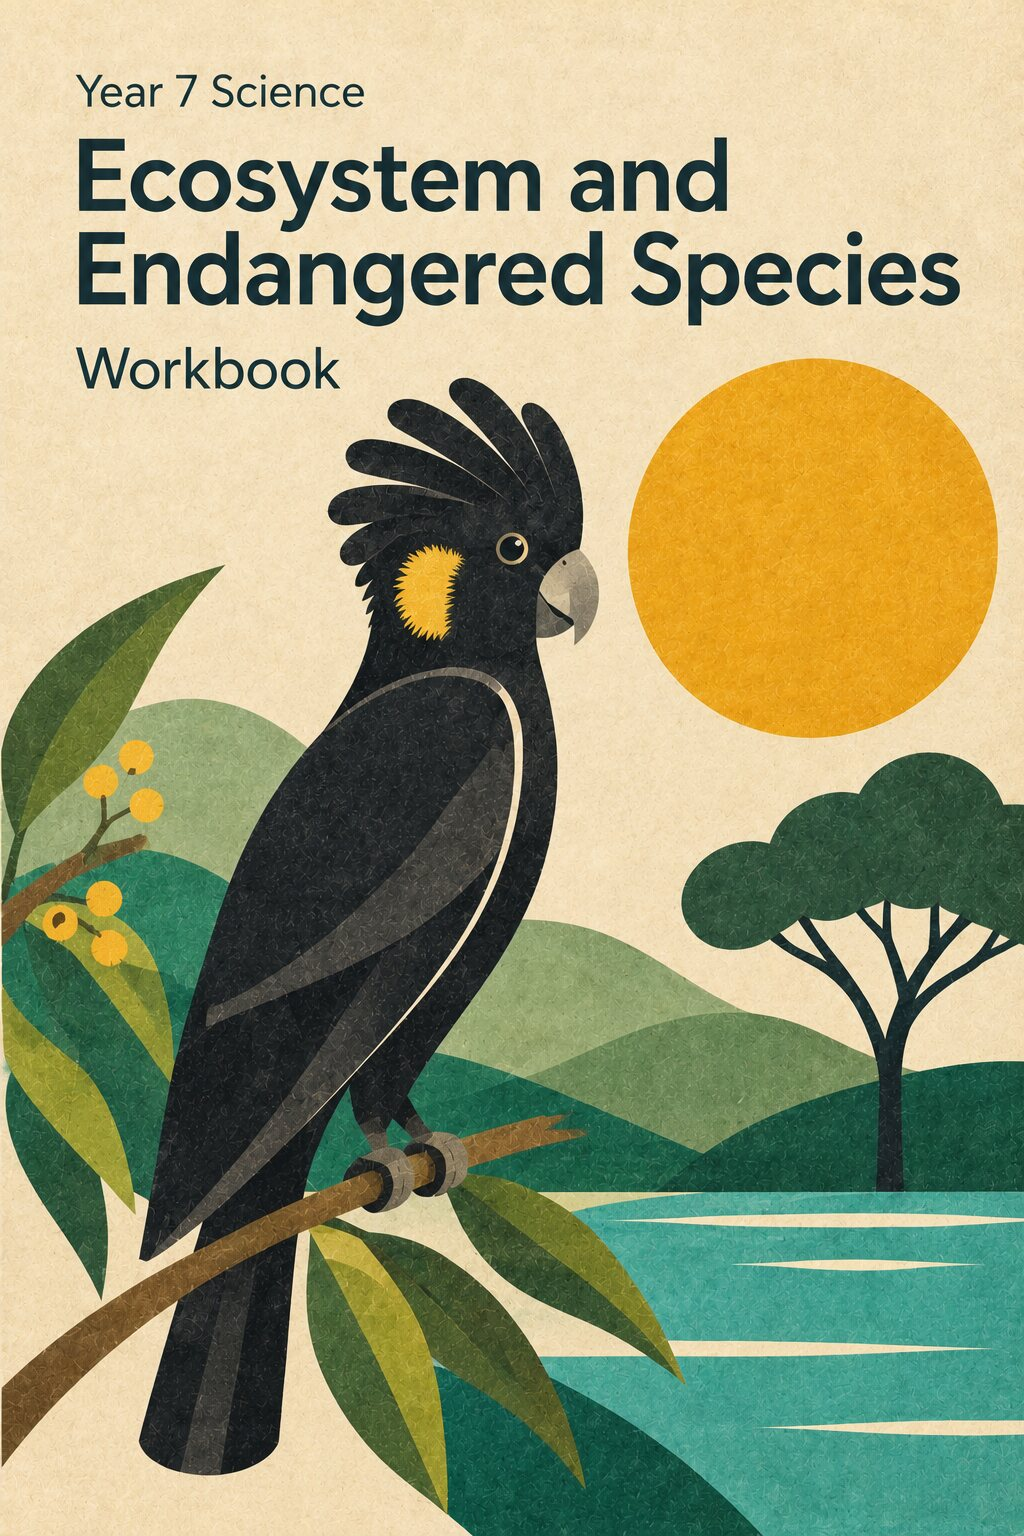
\includegraphics[width=\paperwidth]{../../../covers/ecosystems.jpg}};
  \node[anchor=north east, fill=white, draw=Ink, line width=0.6pt, rounded corners=1.2mm,
        inner xsep=2mm, inner ysep=1.8mm, text width=30mm, font=\headingfont\footnotesize]
    at ([xshift=-4mm, yshift=-4mm]current page.north east)
    {\textbf{Name}\par\vspace{4mm}\hrule\vspace{2mm}\textbf{Class}\par\vspace{4mm}\hrule};
  \node[anchor=south east, fill=white, draw=Ink, line width=0.6pt, rounded corners=1.2mm,
        inner xsep=2.6mm, inner ysep=2mm, font=\headingfont\bfseries, align=right]
    at ([xshift=-4mm, yshift=6mm]current page.south east)
    {Lesson Booklet 3\\[-1pt]{\normalfont\headingfont\scriptsize Lessons 9--11}};
\end{tikzpicture}
\mbox{}
\clearpage

% ---- Inside cover ---------------------------------------------------------
\thispagestyle{plain}
{\headingfont\bfseries\fontsize{22}{26}\selectfont Biodiversity and Ecosystems}\par\vspace{1mm}
{\headingfont\large Lesson Booklet 3 \textbullet\ Lessons 9--11 \textbullet\ Year 7}\par\vspace{1mm}
{\small\itshape VC 2.0: VC2S8U01 \textbullet\ VC2S8U04 \textbullet\ VC2S8I01--I08 \textbullet\ VC2S8H02--H04}\par\vspace{4mm}
\textbf{Teacher}\ \hrulefill\par

\begin{countrybox}{Acknowledgement of Country}
This booklet was created on the unceded Country of the Wurundjeri Woi-wurrung people of the Kulin Nation. We acknowledge Elders past, present and emerging.
\end{countrybox}

\begin{infobox}{How this booklet works}
One section for each lesson. Each opens with its key vocabulary, then:\par\smallskip
\renewcommand{\arraystretch}{1.25}
\begin{tabular}{@{}p{24mm}p{70mm}@{}}
\textbf{Part A} & a reading with comprehension questions \\
\textbf{Part B} & the ideas, worked through \\
\textbf{Part C} & practice on your own \\
\textbf{Part D} & above level: Year 8 extension \\
\end{tabular}

\smallskip
\begin{tabular}{@{}p{24mm}p{70mm}@{}}
\textbf{I do} \tagicon{\icodots{1}} & your teacher works an example (solid frame) \\
\textbf{We do} \tagicon{\icodots{2}} & you try one together (dashed frame) \\
\textbf{Reading} \tagicon{\icoread} & a passage to read (thin frame) \\
\textbf{Above level} \tagicon{\icoup} & extension (double frame) \\
\end{tabular}

\smallskip
Three lesson books. The five labs share a lesson and are in the \textbf{Experiment Booklet}.
\end{infobox}

\clearpage
\markboth{Contents}{Contents}
{\headingfont\bfseries\LARGE Contents}\par\vspace{1mm}\noindent\rule{\linewidth}{0.6pt}\par\vspace{2mm}
\renewcommand{\arraystretch}{1.45}
\begin{tabular}{|C{1.1cm}|L{6.0cm}|C{2.4cm}|}
  \hline\thead{Lesson} & \thead{Title} & \thead{Page} \\ \hline
  1 & \textit{Living or Non-living?} \newline{\footnotesize\itshape + Lab: Is Yeast Alive? (Experiment Booklet)} & Book 1 \\ \hline
  2 & \textit{Classification: Linnaean Levels} & Book 1 \\ \hline
  3 & \textit{Scientific Names and the Six Kingdoms} & Book 1 \\ \hline
  4 & \textit{Dichotomous Keys} \newline{\footnotesize\itshape + Lab: Key the Schoolyard (Experiment Booklet)} & Book 1 \\ \hline
  5 & \textit{Australian Ecosystems and Biodiversity} \newline{\footnotesize\itshape + Lab: Quadrat Survey (Experiment Booklet)} & Book 2 \\ \hline
  6 & \textit{Food Webs and Energy Flow} & Book 2 \\ \hline
  7 & \textit{Ecosystem Services} & Book 2 \\ \hline
  8 & \textit{Adaptations} \newline{\footnotesize\itshape + Lab: Beaks and Food (Experiment Booklet)} & Book 2 \\ \hline
  9 & \hyperlink{lesson.9.1}{Introduced Species} \newline{\footnotesize\itshape + Lab: The Rabbit and Fox Model (Experiment Booklet)} & \hyperlink{lesson.9.1}{p.\ \pageref{sec:9}} \\ \hline
  10 & \hyperlink{lesson.10.1}{Human Impacts on Ecosystems} & \hyperlink{lesson.10.1}{p.\ \pageref{sec:10}} \\ \hline
  11 & \hyperlink{lesson.11.1}{Conservation and Action} & \hyperlink{lesson.11.1}{p.\ \pageref{sec:11}} \\ \hline
  --- & \hyperlink{glossary}{Glossary} & \hyperlink{glossary}{\pageref{sec:glossary}} \\ \hline
\end{tabular}
\renewcommand{\arraystretch}{1}
\clearpage
% ══════════════════════════════════════════════════════════════════════════════
%  BIODIVERSITY AND ECOSYSTEMS — A5 LESSON BOOKLET, LESSONS 9–11
% ══════════════════════════════════════════════════════════════════════════════

% ══════════════════════════════════════════════════════════════════════════════
%  LESSON 9 — INTRODUCED SPECIES
% ══════════════════════════════════════════════════════════════════════════════
\setcounter{section}{8}
\sectiondiv{Introduced Species}{Native, introduced and invasive \textbullet{} Four ways they cause harm \textbullet{} Impact chains}\label{sec:9}
\lessoncodes{VC2S8U04 \textbullet{} VC2S8H03}

\vocabhead
\begin{ctab}
\begin{tabular}{|SW{3.4cm}|W{7.0cm}|}
  \hline\hd & \thead{Word} & \thead{Definition (copy from the slide)} \\ \hline
  & \scaf{\textbf{Native species}\label{voc:native-species}} & \scaf{A species that has always lived in an area, without being brought by people.} \\ \hline
  & \textbf{Introduced species}\label{voc:introduced-species} & \\ \hline
  & \textbf{Invasive species}\label{voc:invasive-species} & \\ \hline
  & \textbf{Predation}\label{voc:predation} & \\ \hline
  & \textbf{Competition}\label{voc:competition} & \\ \hline
  & \textbf{Biological control}\label{voc:biological-control} & \\ \hline
\end{tabular}
\end{ctab}

% ─── PART A ───────────────────────────────────────────────────────────────────
\lessonpart{A}{Reading and comprehension}{Teal}\label{read:9}

\begin{readingbox}{Reading --- Twenty-Four Rabbits}
In 1859 a farmer near Geelong released 24 rabbits so he could hunt them. With plenty of grass and few predators, they bred so fast that within 50 years there were hundreds of millions across Australia. They stripped the land of plants and left the soil bare.

Rabbits are an \textbf{introduced species}: brought to a new place by people, on purpose or by accident. A \textbf{native species}, like the eastern grey kangaroo, has always lived here. Not every introduced species causes trouble, but one that spreads quickly and does real harm is called an \textbf{invasive species}.

Invasive species do harm in four main ways. Through \textbf{predation} they hunt native animals that never evolved to escape them: foxes and cats kill bandicoots and ground-nesting birds. Through \textbf{competition} they take food, water or shelter that native species need: rabbits eat the grass kangaroos rely on. They change habitats, as blackberry does when it smothers creek banks, and they spread diseases.

People fight back with fences, baiting, trapping and \textbf{biological control}: using a living thing, such as a virus, to control a pest. In 1950 the myxoma virus was released and killed most of Australia's rabbits, though survivors slowly became resistant.
\end{readingbox}

\rcreset
\rcq{Why did rabbits spread so quickly in Australia?}{2.5cm}
\rcq{What is the difference between an introduced species and an invasive species?}{2.5cm}
\rcq{Name the four ways invasive species cause harm.}{2.5cm}
\rcq{What is biological control? Give an example.}{2.5cm}
\rcq{Why did the myxoma virus not wipe out rabbits for good?}{2cm}

% ─── PART B ───────────────────────────────────────────────────────────────────
\lessonpart{B}{Theory and examples}{Blue}\label{theory:9}

\subsection{Four Ways of Causing Harm}\label{sub:9.1}

\begin{ctab}
\begin{tabular}{|L{2.3cm}|L{3.8cm}|L{3.9cm}|}
  \hline\thead{Harm} & \thead{What happens} & \thead{Victorian example} \\ \hline
  Predation & Eats native animals with no defences against it & Red fox killing bandicoots \\ \hline
  Competition & Takes food, water or shelter natives need & Rabbits eating kangaroos' grass \\ \hline
  Habitat change & Alters the environment & Blackberry smothering creek banks \\ \hline
  Disease & Carries germs natives cannot fight & Cats spreading toxoplasmosis \\ \hline
\end{tabular}
\end{ctab}

\subsection{Impact Chains}\label{sub:9.2}

\begin{workedex}{European carp}
Carp were released into Victorian rivers in the 1960s. They feed by sucking up mud from the riverbed.

\smallskip
\textbf{Step 1:} feeding stirs up the mud, making the water cloudy and releasing nutrients.\\
\textbf{Step 2:} less light reaches the riverbed, so water plants cannot photosynthesise and die.\\
\textbf{Step 3:} extra nutrients feed algae; when the algae die and rot, oxygen in the water drops.\\
\textbf{Step 4:} native fish such as Murray cod lose shelter, food and oxygen; platypus lose the insect larvae they eat.

\smallskip
One introduced species changed a whole river through a chain of effects: an \textbf{impact chain}.
\end{workedex}

\begin{wedo}{Red foxes}
Red foxes were brought to Victoria in the 1870s for hunting. Trace an impact chain of at least three steps, starting with the foxes eating bandicoots and ground-nesting birds.
\answerbox{5cm}
\end{wedo}

\begin{countrybox}{First Nations perspectives --- Loss of Country and culture}
Before 1835, bettongs, quolls, bandicoots and bush stone-curlews were common on Wurundjeri Woi-wurrung Country. Within decades, sheep, cattle, rabbits, foxes, cats and blackberry arrived together and devastated them. This was not only an environmental loss: many of these animals are totems for particular families, so their loss is a loss of identity and culture. Restoration projects led with Wurundjeri Elders are cultural restoration too.
\end{countrybox}

% ─── PART C ───────────────────────────────────────────────────────────────────
\lessonpart{C}{Practice}{Amber}\label{prac:9}

\task Sort each species as native or introduced to Victoria. For introduced species, give one way it could cause harm: eastern grey kangaroo, European rabbit, red fox, tawny frogmouth, blackberry, common starling, platypus, European carp.
\begin{ctab}
\begin{tabular}{|SW{3.0cm}|W{2.2cm}|W{4.8cm}|}
  \hline\hd & \thead{Species} & \thead{Native or introduced} & \thead{How it could cause harm} \\ \hline
  & \scaf{European rabbit} & \scaf{Introduced} & \scaf{Competition: eats grass native grazers need} \\ \hline
  & & & \\ \hline
  & & & \\ \hline
  & & & \\ \hline
  & & & \\ \hline
  & & & \\ \hline
  & & & \\ \hline
  & & & \\ \hline
\end{tabular}
\end{ctab}

\needspace{10\baselineskip}
\task Native mammals such as bandicoots are easily killed by foxes, but rabbits, also introduced, survive alongside foxes. Suggest why.
\answerbox{5cm}

\needspace{10\baselineskip}
\task Cats were brought to Australia as pets. Explain how a pet can become an invasive species.
\answerbox{5cm}

% ─── PART D ───────────────────────────────────────────────────────────────────
\lessonpart{D}{Above level}{Violet}\label{ext:9}

\begin{yr8box}
These questions go beyond the Year 7 standard.

\medskip
\begin{keepext}
\exttask Evaluate the myxoma virus as a biological control for rabbits: describe how it worked, the evidence that it worked, and one risk of using biological control. (Cane toads are one example of a biological control that went wrong.)
\answerbox{6cm}
\end{keepext}
\begin{keepext}
\exttask Animals on islands are especially at risk from introduced predators. Explain why, and give a Victorian example.
\answerbox{5cm}
\end{keepext}
\end{yr8box}

% ══════════════════════════════════════════════════════════════════════════════
%  LESSON 10 — HUMAN IMPACTS ON ECOSYSTEMS
% ══════════════════════════════════════════════════════════════════════════════
\setcounter{section}{9}
\sectiondiv{Human Impacts on Ecosystems}{Habitat loss \textbullet{} Pollution and eutrophication \textbullet{} Climate change \textbullet{} Threats that combine}\label{sec:10}
\lessoncodes{VC2S8U04 \textbullet{} VC2S8H03}

\vocabhead
\begin{ctab}
\begin{tabular}{|SW{3.4cm}|W{7.0cm}|}
  \hline\hd & \thead{Word} & \thead{Definition (copy from the slide)} \\ \hline
  & \scaf{\textbf{Habitat loss}\label{voc:habitat-loss}} & \scaf{When the place a species lives is destroyed or changed so it can no longer live there.} \\ \hline
  & \textbf{Fragmentation}\label{voc:fragmentation} & \\ \hline
  & \textbf{Pollution}\label{voc:pollution} & \\ \hline
  & \textbf{Eutrophication}\label{voc:eutrophication} & \\ \hline
  & \textbf{Over-harvesting}\label{voc:over-harvesting} & \\ \hline
  & \textbf{Endangered}\label{voc:endangered} & \\ \hline
\end{tabular}
\end{ctab}

% ─── PART A ───────────────────────────────────────────────────────────────────
\lessonpart{A}{Reading and comprehension}{Teal}\label{read:10}

\begin{readingbox}{Reading --- Two-Thirds Gone}
Since European settlement, Victoria has cleared about two-thirds of its native vegetation for farms, towns and roads. The biggest threat to wildlife is \textbf{habitat loss}. When a forest is cleared, the animals that lived there have nowhere to go.

Often the bush is not all cleared, but cut into pieces by roads and paddocks. This \textbf{fragmentation} leaves small, separate patches. Animals in one patch cannot reach mates or food in another, and the edges of each patch get hotter, windier and weedier.

\textbf{Pollution} adds harmful substances to the environment: plastic, pesticides, and fertiliser washed into rivers. Too much fertiliser in water causes \textbf{eutrophication}: algae grow wildly, then die and rot, and the bacteria that rot them use up the oxygen, killing fish.

Climate change brings hotter summers, less snow and bigger fires. \textbf{Over-harvesting} takes fish, animals or plants faster than they can breed. These threats rarely act alone. A species facing several at once can become \textbf{endangered}: at serious risk of dying out.
\end{readingbox}

\rcreset
\rcq{What is the biggest threat to wildlife in Victoria?}{2cm}
\rcq{What is fragmentation, and why is it harmful?}{2.5cm}
\rcq{Explain how fertiliser can kill fish in a lake.}{3cm}
\rcq{Name two effects of climate change on Victorian ecosystems.}{2cm}
\rcq{What does it mean for a species to be endangered?}{2cm}

% ─── PART B ───────────────────────────────────────────────────────────────────
\lessonpart{B}{Theory and examples}{Blue}\label{theory:10}

\subsection{Fragmentation}\label{sub:10.1}

\begin{center}
\begin{fitbox}\begin{tikzpicture}[font=\small]
  \fill[black!25, draw=Ink, line width=0.7pt] (0,0) rectangle (3,3);
  \node[font=\bfseries\small] at (1.5,-0.35) {Reserve A: one block};
  \foreach \x/\y in {4.8/0,6.6/0,4.8/1.8,6.6/1.8}{\fill[black!25, draw=Ink, line width=0.7pt] (\x,\y) rectangle ++(1.5,1.5);
    \draw[Ink, line width=0.5pt, densely dotted] (\x+0.18,\y+0.18) rectangle ++(1.14,1.14);}
  \draw[Ink, line width=0.5pt, densely dotted] (0.18,0.18) rectangle (2.82,2.82);
  \node[font=\bfseries\small] at (6.45,-0.35) {Reserve B: four patches};
\end{tikzpicture}\end{fitbox}
\figcap{Both reserves have the same area. The dotted lines mark the edge zone, which is hotter, windier and weedier.}
\end{center}

\begin{workedex}{Why the patches lose}
Reserve A is one 40\,ha block; Reserve B is four 10\,ha blocks separated by farmland.

\smallskip
In Reserve B, a much bigger share of the bush is edge, where weeds and foxes get in and conditions are harsh. Animals that need a large area, or must cross open farmland to find mates, cannot survive in a 10\,ha patch. So Reserve B supports fewer native species, even with the same total area.
\end{workedex}

\begin{wedo}{Fragmentation}
A new freeway is built through a forest. Suggest two ways to reduce the harm to the forest's animals, and explain how each helps.
\answerbox{5cm}
\end{wedo}

\subsection{Threats that Combine}\label{sub:10.2}

\begin{workedex}{Leadbeater's possum}
Leadbeater's possum, Victoria's animal emblem, nests only in hollows of mountain ash trees more than about 150 years old.

\smallskip
\textbf{Threat 1, habitat loss:} logging has removed most of the old trees with hollows.\\
\textbf{Threat 2, fire:} the 2009 Black Saturday fires burnt nearly half of its remaining habitat.\\
\textbf{Threat 3, climate change:} fires come more often, so regrowing forest burns again before it can grow hollows.

\smallskip
Each threat on its own is serious; together, they push the possum towards extinction.
\end{workedex}

\begin{wedo}{Threats that combine}
The mountain pygmy possum needs deep snow to hibernate under, and bogong moths to eat. Snow cover is shrinking, and drought has cut moth numbers. Explain why these two threats together are worse than either alone.
\answerbox{5cm}
\end{wedo}

\begin{countrybox}{First Nations perspectives --- A long memory of Country}
Written records in Victoria go back only about 190 years. Wurundjeri Woi-wurrung oral histories and knowledge of Country reach back tens of thousands of years, and remember animals and plants that are now gone from an area. When Elders say a species ``should be here'', that is important information for setting goals to restore an ecosystem.
\end{countrybox}

% ─── PART C ───────────────────────────────────────────────────────────────────
\lessonpart{C}{Practice}{Amber}\label{prac:10}

\task Name the main human impact in each case: habitat loss, fragmentation, pollution, climate change, introduced species or over-harvesting.
\begin{ctab}
\begin{tabular}{|SW{6.2cm}|W{3.8cm}|}
  \hline\hd & \thead{Case} & \thead{Main impact} \\ \hline
  & \scaf{A housing estate is built on native grassland} & \scaf{Habitat loss} \\ \hline
  & Fertiliser runoff causes an algal bloom in the Gippsland Lakes & \\ \hline
  & Snow cover in the Victorian Alps has fallen since 1980 & \\ \hline
  & Rabbits eat the grass native grazers need & \\ \hline
  & A freeway splits a forest into two patches & \\ \hline
  & Too many abalone are taken from Port Phillip Bay & \\ \hline
\end{tabular}
\end{ctab}

\needspace{14\baselineskip}
\task Trace the eutrophication of the Gippsland Lakes, one step per part.
\pt{a} Where do the extra nutrients come from?
\answerbox{2.5cm}
\pt{b} What happens to the algae?
\answerbox{2.5cm}
\pt{c} What happens to the water clarity and the water plants?
\answerbox{2.5cm}
\pt{d} What happens to the oxygen and the fish?
\answerbox{2.5cm}

\needspace{10\baselineskip}
\task Choose one Victorian species facing more than one threat. Name it, give two threats, and explain why the combination is worse than either threat alone.
\answerbox{5cm}

% ─── PART D ───────────────────────────────────────────────────────────────────
\lessonpart{D}{Above level}{Violet}\label{ext:10}

\begin{yr8box}
These questions go beyond the Year 7 standard.

\medskip
\begin{keepext}
\exttask A population of eastern barred bandicoots has been cut off in a 15\,ha reserve for 20 years. Explain two risks that small, isolated populations face. Use the terms \emph{genetic diversity} and \emph{inbreeding}.
\answerbox{6cm}
\end{keepext}
\begin{keepext}
\exttask Explain why losing biodiversity can make it harder for the world to deal with other problems, such as climate change or supplies of fresh water.
\answerbox{5cm}
\end{keepext}
\end{yr8box}

% ══════════════════════════════════════════════════════════════════════════════
%  LESSON 11 — CONSERVATION AND ACTION
% ══════════════════════════════════════════════════════════════════════════════
\setcounter{section}{10}
\sectiondiv{Conservation and Action}{In-situ and ex-situ \textbullet{} A Victorian success story \textbullet{} What we can do}\label{sec:11}
\lessoncodes{VC2S8U04 \textbullet{} VC2S8H03 \textbullet{} VC2S8H04}

\vocabhead
\begin{ctab}
\begin{tabular}{|SW{3.4cm}|W{7.0cm}|}
  \hline\hd & \thead{Word} & \thead{Definition (copy from the slide)} \\ \hline
  & \scaf{\textbf{Conservation}\label{voc:conservation}} & \scaf{Protecting species and ecosystems so they survive into the future.} \\ \hline
  & \textbf{In-situ}\label{voc:in-situ} & \\ \hline
  & \textbf{Ex-situ}\label{voc:ex-situ} & \\ \hline
  & \textbf{Captive breeding}\label{voc:captive-breeding} & \\ \hline
  & \textbf{Reintroduction}\label{voc:reintroduction} & \\ \hline
  & \textbf{Habitat corridor}\label{voc:habitat-corridor} & \\ \hline
\end{tabular}
\end{ctab}

% ─── PART A ───────────────────────────────────────────────────────────────────
\lessonpart{A}{Reading and comprehension}{Teal}\label{read:11}

\begin{readingbox}{Reading --- Back from the Brink}
By 1989 the eastern barred bandicoot was gone from the wild in mainland Victoria. Foxes, cats and the loss of its grassland habitat had wiped it out, except for a few animals in captivity. Its story since then is one of Australia's great \textbf{conservation} successes.

Conservation works in two ways. \textbf{In-situ} conservation (``in place'') protects species where they live: national parks, fences that keep out foxes and cats, and \textbf{habitat corridors}, strips of bush that join separate patches so animals can move between them. \textbf{Ex-situ} conservation (``out of place'') protects species away from the wild: zoos, seed banks, and \textbf{captive breeding}, where animals are bred in safety.

The bandicoot recovery used both. Zoos Victoria and Healesville Sanctuary bred bandicoots in captivity. Meanwhile, predator-free areas were made on the mainland and on fox-free islands, ready for their \textbf{reintroduction}: releasing animals back into the wild. In 2021 it became the first in Australia to be moved from ``extinct in the wild'' to ``endangered''.
\end{readingbox}

\rcreset
\rcq{Why had the eastern barred bandicoot disappeared from the wild?}{2.5cm}
\rcq{What is the difference between in-situ and ex-situ conservation?}{2.5cm}
\rcq{What is a habitat corridor, and how does it help animals?}{2.5cm}
\rcq{What had to be ready before bandicoots could be reintroduced?}{2.5cm}
\rcq{What change in the bandicoot's status happened in 2021?}{2cm}

% ─── PART B ───────────────────────────────────────────────────────────────────
\lessonpart{B}{Theory and examples}{Blue}\label{theory:11}

\subsection{In-situ and Ex-situ}\label{sub:11.1}

\begin{ctab}
\begin{tabular}{|L{4.9cm}|L{4.9cm}|}
  \hline\thead{In-situ (in place)} & \thead{Ex-situ (out of place)} \\ \hline
  National parks and reserves & Captive breeding in zoos \\ \hline
  Habitat corridors & Seed banks \\ \hline
  Fox and cat control & Freezing eggs, sperm or tissue \\ \hline
  Laws protecting native vegetation & Growing rare plants in nurseries \\ \hline
\end{tabular}
\end{ctab}

\begin{workedex}{Evaluating a strategy: habitat corridors}
\textbf{How it works:} planting strips of native bush to join isolated patches.\\
\textbf{Evidence:} connected patches hold more bird species than isolated patches of the same size; powerful owls use creek corridors to move through Melbourne.\\
\textbf{Advantages:} cheaper than buying land; lets animals find mates and food.\\
\textbf{Limitations:} weeds, fire and disease can spread along corridors too; narrow corridors are not used by some species.\\
\textbf{Judgement:} effective, especially for animals that move a lot, but best used alongside reserves and predator control.
\end{workedex}

\begin{wedo}{Evaluating a strategy: captive breeding}
Use the same headings (how it works, an advantage, a limitation, a judgement) to evaluate captive breeding.
\answerbox{6cm}
\end{wedo}

\begin{countrybox}{First Nations perspectives --- The oldest conservation system}
First Nations peoples have cared for Country and its biodiversity for at least 65\,000 years. Caring for Country is a living system of land management, not a thing of the past. Indigenous Protected Areas, managed by First Nations communities, now make up the largest share of Australia's protected land. For Wurundjeri Woi-wurrung people, managing Country again is also about self-determination and healing.
\end{countrybox}

% ─── PART C ───────────────────────────────────────────────────────────────────
\lessonpart{C}{Practice}{Amber}\label{prac:11}

\task Rank these strategies from 1 (most effective) to 6 (least effective), in your opinion, and label each in-situ or ex-situ.
\begin{ctab}
\begin{tabular}{|SW{5.6cm}|Z{2.0cm}|Z{1.8cm}|}
  \hline\hd & \thead{Strategy} & \thead{In-situ or ex-situ} & \thead{Rank} \\ \hline
  & \scaf{Create a new national park} & \scaf{In-situ} & \\ \hline
  & Run a captive breeding program & & \\ \hline
  & Plant corridors between bush patches & & \\ \hline
  & Freeze seeds in a seed bank & & \\ \hline
  & Pass a law banning a harmful pesticide & & \\ \hline
  & Teach the community about pest species & & \\ \hline
\end{tabular}
\end{ctab}
Justify your top choice.
\answerbox{4cm}

\needspace{14\baselineskip}
\task The eastern barred bandicoot recovery program bred bandicoots at zoos, then released them into fox-free enclosures and islands.
\pt{a} Is this in-situ, ex-situ or both? Explain.
\answerbox{4cm}
\pt{b} By 2022 there were more than 1500 bandicoots in the wild. What does this tell you about the program? What worries remain?
\answerbox{5cm}

\needspace{14\baselineskip}
\task Design a conservation action your school or community could take for native wildlife in Melbourne's northern suburbs.
\pt{a} What is the action?
\answerbox{2.5cm}
\pt{b} How would it help native species? Use an idea from this unit.
\answerbox{4cm}
\pt{c} Give one limitation of your action.
\answerbox{3cm}

% ─── PART D ───────────────────────────────────────────────────────────────────
\lessonpart{D}{Above level}{Violet}\label{ext:11}

\begin{yr8box}
These questions go beyond the Year 7 standard.

\medskip
\begin{keepext}
\exttask The EPBC Act is Australia's main law for protecting threatened species. A 2020 review found it ``not fit for purpose'', because biodiversity keeps falling. Explain what the law is meant to do, what evidence suggests it is failing, and one improvement you would make.
\answerbox{6cm}
\end{keepext}
\begin{keepext}
\exttask Some scientists propose bringing Tasmanian devils back to mainland Victoria to control foxes and cats. Give one ecological benefit, one concern farmers or communities might raise, and say who you think should decide, and why.
\answerbox{6cm}
\end{keepext}
\end{yr8box}

\clearpage
{\headingfont\bfseries\Large Final reflection}\par\vspace{0.5mm}\noindent\rule{\linewidth}{0.6pt}\par\vspace{2mm}
What is the one idea from this unit that most changed how you think about the living world? Write a paragraph.
\answerbox{11cm}
\clearpage\markboth{Glossary}{Glossary}\hypertarget{glossary}{}\pdfbookmark[1]{Glossary}{glossarybm}
{\headingfont\bfseries\LARGE Glossary}\label{sec:glossary}\par\vspace{1mm}\noindent\rule{\linewidth}{0.6pt}\par
{\small Every key word in this booklet and the page it is introduced on.}\par\smallskip
\renewcommand{\arraystretch}{1.3}
\begin{longtable}{|>{\RaggedRight}p{34mm}|p{9mm}|p{\dimexpr\linewidth-43mm-6\tabcolsep-4\arrayrulewidth-1pt\relax}|}
\hline \rule{0pt}{4mm}\headingfont\bfseries Word & \headingfont\bfseries Page & \headingfont\bfseries In my own words \\ \hline \endhead
  Biological control & \pageref{voc:biological-control} & \\ \hline
  Captive breeding & \pageref{voc:captive-breeding} & \\ \hline
  Competition & \pageref{voc:competition} & \\ \hline
  Conservation & \pageref{voc:conservation} & \\ \hline
  Endangered & \pageref{voc:endangered} & \\ \hline
  Eutrophication & \pageref{voc:eutrophication} & \\ \hline
  Ex-situ & \pageref{voc:ex-situ} & \\ \hline
  Fragmentation & \pageref{voc:fragmentation} & \\ \hline
  Habitat corridor & \pageref{voc:habitat-corridor} & \\ \hline
  Habitat loss & \pageref{voc:habitat-loss} & \\ \hline
  In-situ & \pageref{voc:in-situ} & \\ \hline
  Introduced species & \pageref{voc:introduced-species} & \\ \hline
  Invasive species & \pageref{voc:invasive-species} & \\ \hline
  Native species & \pageref{voc:native-species} & \\ \hline
  Over-harvesting & \pageref{voc:over-harvesting} & \\ \hline
  Pollution & \pageref{voc:pollution} & \\ \hline
  Predation & \pageref{voc:predation} & \\ \hline
  Reintroduction & \pageref{voc:reintroduction} & \\ \hline
\end{longtable}
\padtofour
\end{document}
